\chapter{RESULTADOS}
%Título Capítulo 6
Alguns experimentos para diferentes tempos de simulação foram realizados, tanto no modelo de configuração euleriana proposto nessa dissertação, como no código lagrageano PySPH utilizado como referência. Os resultados mais significativos encontrados, utilizando o modelo de híbrido, são analisados na Seção \ref{Hibri}, enquanto aqueles obtidos por meio do código PySPH são apresentados na Seção \ref{REPy}.  Um comparativo entre os resultados encontrados nesses dois método é discutido na Seção \ref{Comparacao}.  


\section{ANÁLISE DOS RESULTADOS OBTIDOS} \label{Hibri}

 A estratégia utilizada para a obtenção dos resultados, utilizando o código desenvolvido nesse trabalho, consistiu em determinar valores médios para as velocidades e as alturas atingidas pelo perfil da coluna d'água. Cada intervalo de tempo adotado foi incrementado, inicialmente, em $t= 0,05s$ com o intuito de compor os valores médios. Essa estratégia tornou possível um bom tratamento e análise dos resultados, uma vez que eliminou valores que prejudicavam a representação gráfica. Além disso, o comprimento do tanque foi discretizado em intervalos de $x=0,2 \ m$ o que permitiu a visualização dos perfis nos diversos ponto do escoamento e em todos os tempos de simulação, ou seja, até atingir o estado de regime permanente do escoamento.
 
 O primeiro ponto adotado para visualizar o escoamento foi $x= 0,2 \ m$, com tempo total de simulação de aproximadamente $t = 7,5s$, momento em que as velocidades e as alturas iniciam um estado de regime permanente, Figura \ref{perfil2s}.
 
 Nota-se nessa figura o aumento das velocidades e a diminuição das alturas no exato momento em que se inicia o movimento da coluna d'água, o que representou, com boa fidelidade, o fenômeno físico. Logo após, as velocidades, bem como as alturas, tendem a se estabilizarem indicando que a coluna d'água ainda está percorrendo a extensão do canal. Em seguida, há uma acentuada queda nas velocidades, acompanhada por uma elevação no perfil das alturas, o que confere com o momento em que o fluido colide com o muro localizado no lado direito do canal, $L=4 \ m$, formando o \textit{sloshing}, fenômeno esse que pode ser visto em detalhes no trabalho de \citeonline{Carbajal}. Após isso, tanto as velocidades como as alturas tendem a oscilar, devido às colisões, em menores escalas, com os muros laterais, até atingirem o estado, aparentemente, estacionário. 
 
 \begin{figure}[H]
 	\centering
 	% 	\fbox{\includegraphics[scale=.6]{perfil2s.jpg}}
 	\includegraphics[scale=1]{figuras/perfil2s.jpg}
 	\caption{\textsc{Perfil da velocidade média $u$ e a altura da coluna d'água $h$ para o ponto $x=0,2 \ m$}}
 	\vspace{-0.1cm}
 	\legend{FONTE: Programa do autor usando as equações de Águas Rasas}
 	\label{perfil2s}
 \end{figure}
 
 Uma análise semelhante ao que foi feito anteriormente pode ser realizada na Figura \ref{perfil04s}. No entanto, percebe-se que as velocidades são maiores, já que o ponto adotado para compor as médias é agora de $x= 0,4 \ m$, ou seja, valores diferentes compõem as médias. Assim, é possível notar os momentos de colisão com os muros e a formação do \textit{sloshing} numa posição diferente do tanque.
 
 Comparando a Figura \ref{perfil2s} com a Figura \ref{perfil04s} observa-se que as velocidades têm médias iniciais nulas, o mesmo ocorrendo com as alturas da coluna d'água que permanecem com  $h=2 \ m$. Esse fato ocorre pois, nos primeiros instantes do escoamento, tanto $u$ como $h$ são determinados pelas equações (\ref{solzMod1}) e (\ref{soluMod1}). 
 
 \begin{figure}[H]
 	\centering
 	% 	\fbox{\includegraphics[scale=.6]{perfil04s.jpg}}
 	\includegraphics[scale=1]{figuras/perfil04s.jpg}
 	\caption{\textsc{Perfil da velocidade média $u$ e a altura da coluna d'água $h$ para o ponto $x=0,4 \ m$} }
 	\vspace{-0.1cm}
 	\legend{FONTE: Programa do autor usando as equações de Águas Rasas}
 	\label{perfil04s}
 \end{figure}
 
 Considerando as médias em um ponto mais distante da barragem,  $x= 1,0 \ m$, Figura \ref{perfil0s}, alguns fenômenos físicos no início do movimento deixam de ser capturados. Observa-se que as velocidades médias são maiores do que as anteriores, aproximadamente $u=3 \ m/s$, já neste ponto a massa líquida está percorrendo o tanque ainda sob ação da queda. O mesmo ocorre com as alturas, onde não estão mais claros os perfis iniciais da barragem antes de sua ruptura. Nota-se também, que há pouca captura dos fenômenos formados no momento em que o fluido colide com os muros.
 
 \begin{figure}[H]
 	\centering
 	% 	\fbox{\includegraphics[scale=.6]{perfil10s.jpg}}
 	\includegraphics[scale=1]{figuras/perfil10s.jpg}
 	\caption{\textsc{Perfil da velocidade média $u$ e a altura da coluna d'água $h$ para o ponto $x=1,0 \ m$}}
 	\vspace{-0.1cm}
 	\legend{FONTE: Programa do autor usando as equações de Águas Rasas}
 	\label{perfil0s}
 \end{figure}
 
 Ainda dentro dessa linha de raciocínio, para Figura \ref{perfil4s}, localizada no ponto $x= 1,4 \ m$, observa-se que a velocidade média atinge o seu máximo, $u=8,5 \ m/s$, quando a altura do fluido ainda é próxima de zero. Isso ocorre devido à posição em que o ponto se encontra, já que nesse caso as médias são calculadas por meio das equações (\ref{solzMod}) e (\ref{soluMod}).
 
 \begin{figure}[H]
 	\centering
 	% 	\fbox{\includegraphics[scale=.6]{perfil14s.jpg}}
 	\includegraphics[scale=1]{figuras/perfil14s.jpg}
 	\caption{\textsc{Perfil da velocidade média $u$ e a altura da coluna d'água $h$ para o ponto $x=1,4 \ m$}}
 	\vspace{-0.1cm}
 	\legend{FONTE: Programa do autor usando as equações de Águas Rasas}
 	\label{perfil4s}
 \end{figure}
 
 No caso das Figuras \ref{perfi20s} e \ref{perfi30s} os pontos estão localizados em $x= 2,0 \ m$ e $x= 3,0 \ m$, respectivamente. Essas localizações mostraram-se pouco eficientes na captura dos fenômenos formados, já encontram-se afastadas tanto da barragem como do muro direito. No entanto, serviram para verificar a funcionalidade do código implementado, pois as médias, nos instantes iniciais do escoamento, foram calculadas por intermédio das equações (\ref{solzMod2}) e (\ref{soluMod2}).
 
 \begin{figure}[H]
 	\centering
 	% 	\fbox{\includegraphics[scale=.6]{perfil20s.jpg}}
 	\includegraphics[scale=1]{figuras/perfil20s.jpg}
 	\caption{\textsc{Perfil da velocidade média $u$ e a altura da coluna d'água $h$ para o ponto $x=2,0 \ m$}}
 	\vspace{-0.1cm}
 	\legend{FONTE: Programa do autor usando as equações de Águas Rasas}
 	\label{perfi20s}
 \end{figure}
 
 \begin{figure}[H]
 	\centering
 	% 	\fbox{\includegraphics[scale=.6]{perfil30s.jpg}}
 	\includegraphics[scale=1]{figuras/perfil30s.jpg}
 	\caption{\textsc{Perfil da velocidade média $u$ e a altura da coluna d'água $h$ para o ponto $x=3,0 \ m$}}
 	\vspace{-0.1cm}
 	\legend{FONTE: Programa do autor usando as equações de Águas Rasas}
 	\label{perfi30s}
 \end{figure}
 
 Outra forma de análise que pode ser realizada no experimento é verificar o comportamento da massa líquida em certos tempos de simulação, já que os resultados determinados pelo modelo, conforme comentado anteriormente, também foram incrementados a cada $t=0,05s$. Assim, se for considerado o perfil de altura da coluna d'água, pode-se analisar seu comportamento durante o percurso dentro do tanque, como mostra a Figura \ref{Alt01s} que simula o escoamento no início do movimento $t=0,05s$.
 
 \begin{figure}[H]
 	\centering
 	% 	\fbox{\includegraphics[scale=.6]{perfil30s.jpg}}
 	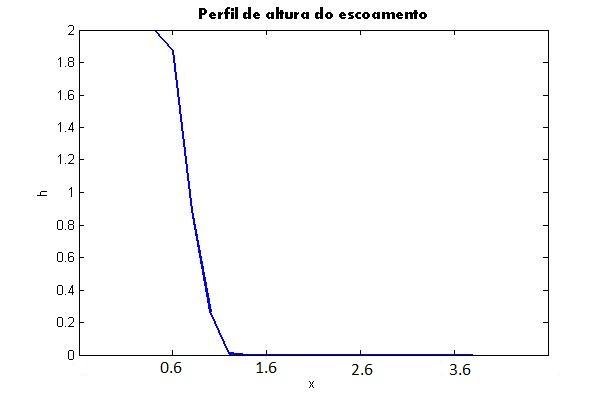
\includegraphics[scale=1]{figuras/Alt01s.jpg}
 	\caption{\textsc{Perfil de altura da coluna d'água $h$ para o tempo $t=0,05s$}}
 	\vspace{-0.1cm}
 	\legend{FONTE: Programa do autor usando as equações de Águas Rasas}
 	\label{Alt01s}
 \end{figure}
 Nota-se nessa figura que o perfil do reservatório está bem definido $h=2 \ m$ e logo após a posição $x=0,6 \ m$ inicia-se o escoamento, elevando a altura da coluna d'água formando a frente de onda.
 
 Na Figura \ref{alt1s} o tempo de simulação é de $t=0,1s$. Nesse instante de tempo a coluna d'água atinge um ponto mais distante da barragem, $x=1,6 \ m$ e já há uma  diminuição na altura do reservatório.
 \begin{figure}[H]
 	\centering
 	% 	\fbox{\includegraphics[scale=.6]{perfil30s.jpg}}
 	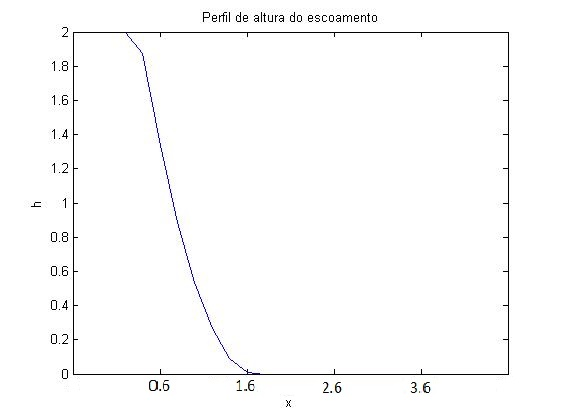
\includegraphics[scale=1]{figuras/alt1s.jpg}
 	\caption{\textsc{Perfil de altura da coluna d'água $h$ para o tempo $t=0,1s$}}
 	\vspace{-0.1cm}
 	\legend{FONTE: Programa do autor usando as equações de Águas Rasas}
 	\label{alt1s}
 \end{figure}
 
 Percebe-se na Figura \ref{Alt2s} que o perfil da superfície livre, no tempo $t=0,2s$, já se aproxima do resultado mostrado na Figura \ref{ondalonga} indicando que profundidade está se tornado constante em toda distância do tanque.
 \begin{figure}[H]
 	\centering
 	% 	\fbox{\includegraphics[scale=.6]{perfil30s.jpg}}
 	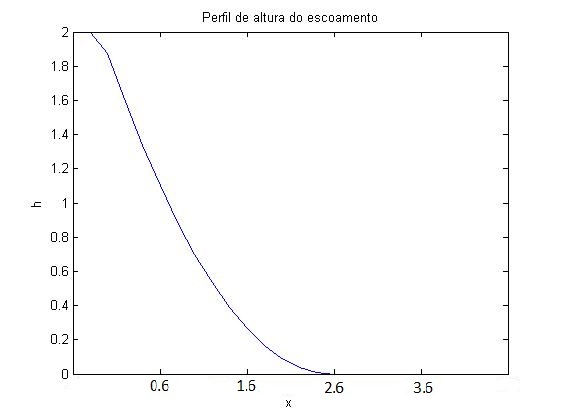
\includegraphics[scale=1]{figuras/Alt2s.jpg}
 	\caption{\textsc{Perfil de altura da coluna d'água $h$ para o tempo $t=0,2s$}}
 	\vspace{-0.1cm}
 	\legend{FONTE: Programa do autor usando as equações de Águas Rasas}
 	\label{Alt2s}
 \end{figure}
 
 A formação do \textit{sloshing} pode ser notado na Figura \ref{Alt35s} quando a coluna d'água atinge o muro no lado direito do tanque logo após o tempo $t=0,35s$.
 \begin{figure}[H]
 	\centering
 	% 	\fbox{\includegraphics[scale=.6]{perfil30s.jpg}}
 	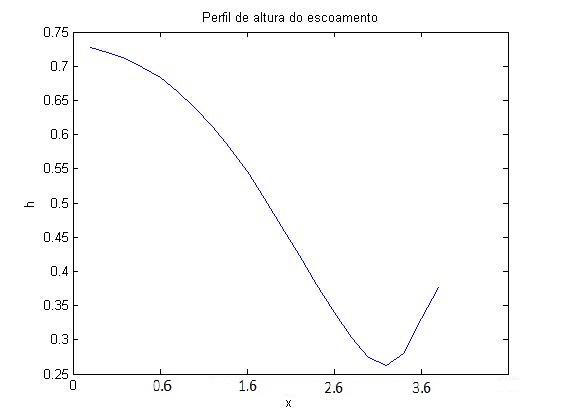
\includegraphics[scale=1]{figuras/Alt35s.jpg}
 	\caption{\textsc{Perfil de altura da coluna d'água $h$ e a formação do \textit{sloshing} no tempo $t=0,35s$}}
 	\vspace{-0.1cm}
 	\legend{FONTE: Programa do autor usando as equações de Águas Rasas}
 	\label{Alt35s}
 \end{figure}
 
 Após a formação do \textit{sloshing} a frente de onda atinge uma altura próxima de $h=1,2 \ m$ e começa a retornar seu percurso até atingir o muro lateral esquerdo, como pode ser observado na Figura \ref{Alt75s}. Logo após, a altura da frente de onda diminui, $h=0,6 \ m$ se aproximando mais ainda do muro esquerdo, Figura \ref{Alt120s}.
  
 \begin{figure}[H]
 	\centering
 	% 	\fbox{\includegraphics[scale=.6]{perfil30s.jpg}}
 	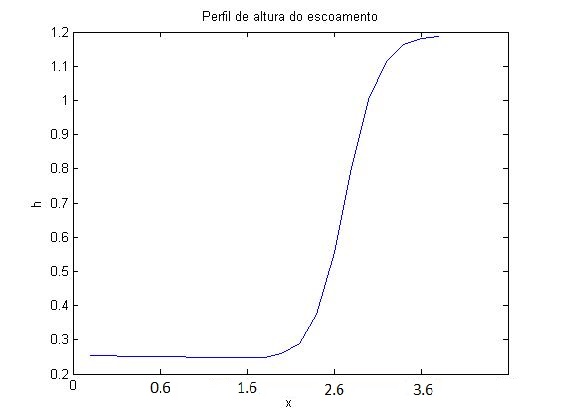
\includegraphics[scale=1]{figuras/Alt75s.jpg}
 	\caption{\textsc{Perfil de altura da coluna d'água $h$ para o tempo $t=0,75s$}}
 	\legend{FONTE: Programa do autor usando as equações de Águas Rasas}
 	\label{Alt75s}
 \end{figure}
 
  \begin{figure}[H]
  	\centering
  	% 	\fbox{\includegraphics[scale=.6]{perfil30s.jpg}}
  	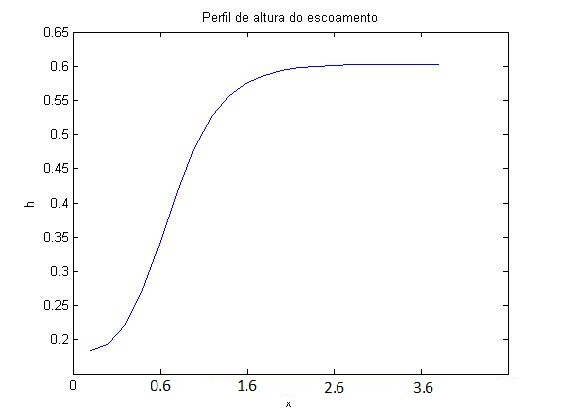
\includegraphics[scale=1]{figuras/Alt120s.jpg}
  	\caption{\textsc{Perfil de altura da coluna d'água $h$ para o tempo $t=1,2s$}}
  	\vspace{-0.1cm}
  	\legend{FONTE: Programa do autor usando as equações de Águas Rasas}
  	\label{Alt120s}
  \end{figure}
  
  Depois de colidir com o muro no lado esquerdo do tanque a frente de onda retorna seu movimento para direção do escoamento até colidir novamente com o muro do lado direito. Esse movimento se repete até que as velocidade se anulem e a profundidade se torne constante. A Figura \ref{Alt350s} mostra a altura da frente de onda oscilando entre $h=0,48 \ m$ e $h=0,52 \ m$ no tempo de simulação $t=3,5s$.
  \begin{figure}[H]
  	\centering
  	% 	\fbox{\includegraphics[scale=.6]{perfil30s.jpg}}
  	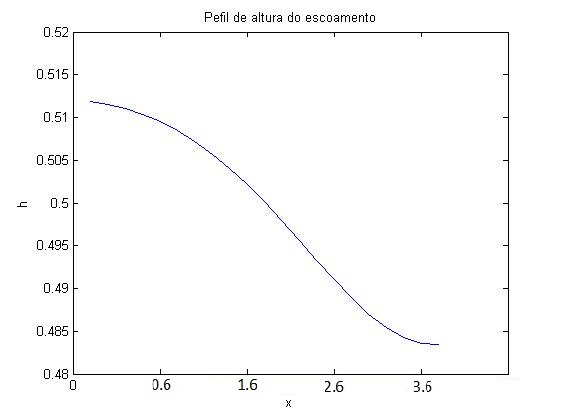
\includegraphics[scale=1]{figuras/Alt350s.jpg}
  	\caption{\textsc{Oscilação do frente de onda no tempo $t=3,5s$}}
  	\legend{FONTE: Programa do autor usando as equações de Águas Rasas}
  	\label{Alt350s}
  \end{figure}   	      
 
   
%------------------------------------------------------------------------------------------------------------------------------------------------------
\section{ANÁLISE DOS RESULTADOS OBTIDOS NO PySPH} \label{REPy}

Devido à complexidade dos cálculos que envolvem o método SPH na formação dos núcleos e suas vizinhanças, na construção das fronteiras, sejam elas fantasmas ou dinâmicas, entre outros, exige uma capacidade de processamento de máquina considerável. A utilização do código PySPH não modificou essa realidade, mesmo os cálculos mais complexos sendo realizados em Cython. O tempo de processamento gasto para simular o exemplo citado na Seção \ref{py} foi de aproximadamente $30$ minutos em um computador pessoal com velocidade de processamento de $1.6 \  GHz$ e $2 \ GB$ de memória RAM. Esse tempo sobe para mais de $10h$ quando a suavização do núcleo diminui para $h=0,0156 \ m$, resultando em $28.056$ partículas para representar o fluido e $1.669$ partículas para formar as fronteiras.

Apesar do tempo gasto na simulação ser alto, o código foi capaz de representar o fenômeno da ruptura de barragens, uma vez que sua eficiência já havia sido comprovada no trabalho de \citeonline{Ramachandran2010}. No entanto, alguns parâmetros como tempo de simulação, tamanho do núcleo e tipo de fronteira foram alterados nesse experimento.

O primeiro resultado obtido foi para o início do escoamento $t=0,01s$, onde os valor da densidade da massa líquida já começam a sofrer alterações, como pode ser visto na Figura \ref{fig:pysph01s}.   

\begin{figure}[H]
	\centering
	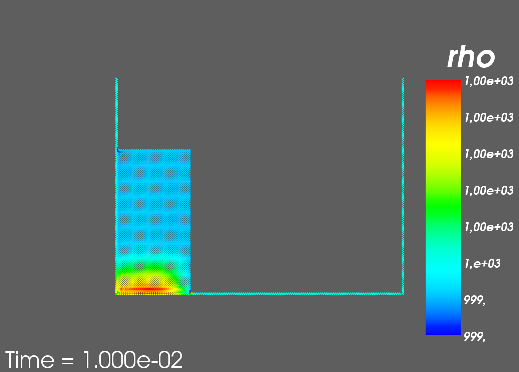
\includegraphics[scale=0.5]{figuras/pysph01s.png}
	\caption{\textsc{Mudanças nos valores da densidade no início da simulação $t=0,01s$}}
	\vspace{-0.1cm}
	\legend{FONTE: Simulação do autor utilizando o código PySPH}
	\label{fig:pysph01s}
\end{figure}

Para o tempo $t=0,1s$ a massa líquida já começa a se deslocar, formando a frente de onda. No entanto, divido a ação das partículas que compõem o fundo do canal, há uma elevação nesse ponto, Figura \ref{fig:pysph1s}. Como alternativa para o problema, a solução poderia ser refinado considerando-se um maior número de partículas compondo o fluido, mas o esforço computacional seria maior. 

\begin{figure}[H]
	\centering
	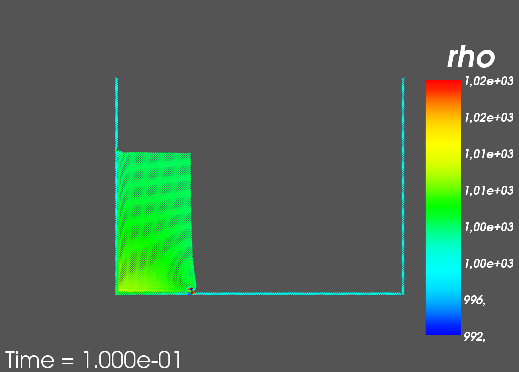
\includegraphics[scale=0.5]{figuras/pysph1s.png}
	\caption{\textsc{Alteração nos valores da densidade próximo ao leito $t=0,1s$}}
	\vspace{-0.1cm}
	\legend{FONTE: Simulação do autor utilizando o código PySPH}
	\label{fig:pysph1s}
\end{figure}

Na Figura \ref{fig:pysph2s} a ação das partículas fantasmas se torna mais evidente. Além disso, nota-se que o perfil da superfície livre não está escoando e sim descendo, com algumas partículas ainda presas na lateral esquerda do tanque. 

\begin{figure}[H]
	\centering
	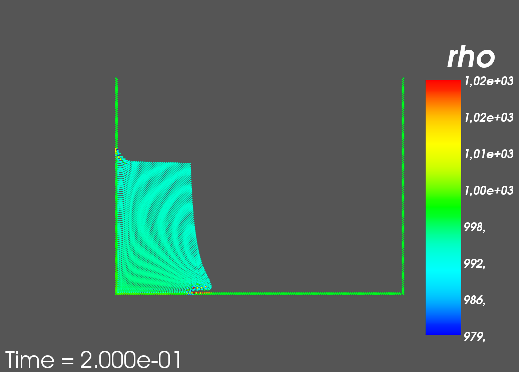
\includegraphics[scale=0.5]{figuras/pysph2s.png}
	\caption{\textsc{Evolução da coluna d'água sobre o leito $t=0,2s$}}
	\vspace{-0.1cm}
	\legend{FONTE: Simulação do autor utilizando o código PySPH}
	\label{fig:pysph2s}
\end{figure}

Os efeitos das fronteira continuam agindo sobre o escoamento, Figura \ref{fig:pysph4s}, afastando a frente de onda do fundo do tanque. Esse efeito é justamente a forma como deve atuar as fronteiras, ou seja, repelir evitando que as partículas do fluido passem para fora do tanque. No entanto, esse efeito deve ser atenuado.  

\begin{figure}[H]
	\centering
	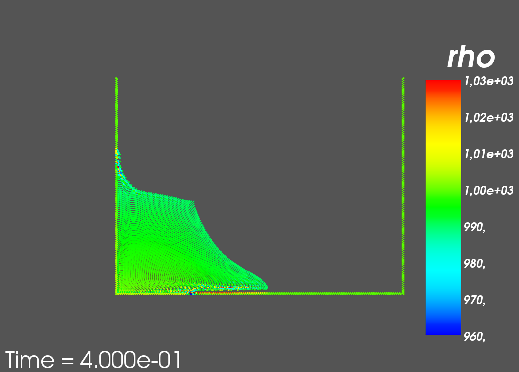
\includegraphics[scale=0.5]{figuras/pysph4s.png}
	\caption{\textsc{Efeito do método da fronteira dinâmica sobre o fluido $t=0,4s$}}
	\vspace{-0.1cm}
	\legend{FONTE: Simulação do autor utilizando o código PySPH}
	\label{fig:pysph4s}
\end{figure}

Na realização desta simulação, o fluido atinge a lateral direita do tanque no tempo $t=0,75s$ iniciando a formação do \textit{sloshing}, conforme mostram as Figuras \ref{fig:pysph75s} e \ref{fig:pysph8s}.  

\begin{figure}[H]
	\centering
	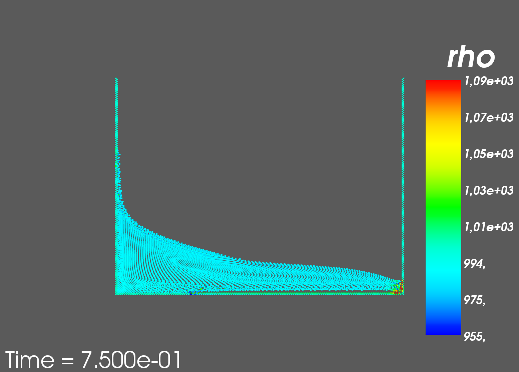
\includegraphics[scale=0.5]{figuras/pysph75s.png}
	\caption{\textsc{Choque da coluna d'água com o muro direito e alteração nos valores da densidade $t=0,75s$}}
	\vspace{-0.1cm}
	\legend{FONTE: Simulação do autor utilizando o código PySPH}
	\label{fig:pysph75s}
\end{figure}

\begin{figure}[H]
	\centering
	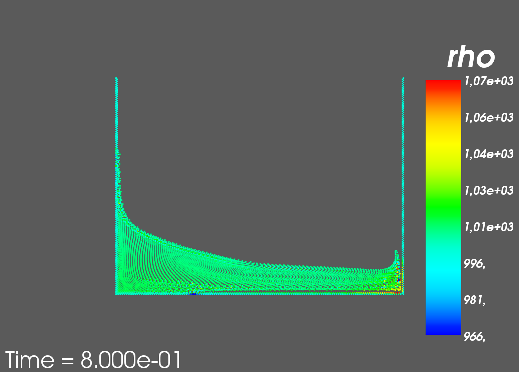
\includegraphics[scale=0.5]{figuras/pysph8s.png}
	\caption{\textsc{Formação do \textit{sloshing} após a colisão som o muro direito $t=0,8s$}}
	\vspace{-0.1cm}
	\legend{FONTE: Simulação do autor utilizando o código PySPH}
	\label{fig:pysph8s}
\end{figure}

A simulação é finalizada no tempo $t=1s$, quando a crista formada pelo \textit{sloshing} ainda está se elevando, como mostra a Figura \ref{fig:pysphfim}. Notou-se que há uma certa desconformidade nos resultados, uma vez que a crista continua subindo e não há o retorno da massa líquida como  era esperado. Dessa forma, a simulação deixou de fazer sentido.

\begin{figure}[H]
	\centering
	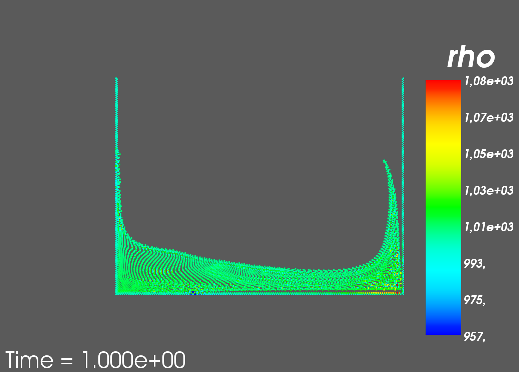
\includegraphics[scale=0.5]{figuras/pysphfim.png}
	\caption{\textsc{Configuração final da simulação $t=1s$}}
	\vspace{-0.1cm}
	\legend{FONTE: Simulação do autor utilizando o código PySPH}
	\label{fig:pysphfim}
\end{figure}


%-------------------------------------------------------------------------------------------------------------------------------------------------------
\section{COMPARAÇÃO DOS RESULTADOS} \label{Comparacao}

A proposta desta seção, conforme exposto nos objetivos desta dissertação, é de fazer comparativos entre os resultados obtidos pelo modelo híbrido desenvolvido e aqueles encontrados por meio do código PySPH. Pode-se dizer, inicialmente, que o modelo foi capaz de simular a ruptura da barragem hipotética utilizada como problema base, assim como ocorreu no PySPH. No entanto, esse comparativo foi prejudicado devido à forma como o código PySPH apresentou seus resultados. Mesmo alterando os parâmetros que deveriam ser mostrados, como as velocidades, a visualização final era sempre o perfil da densidade. Isso dificultou o comparativo, já que no modelo desenvolvido foram obtidos os parâmetros de velocidade e altura da superfície livre.

Em ambos os códigos, um comparativo que pode ser feito é a respeito do tempo gasto para simular o problema proposto. No modelo híbrido, o tempo gasto é de menos de $t=2$ minutos para simular, aproximadamente, $t=7,5s$ de escoamento. Isso ocorre por se tratar de um código unidimensional e com poucos cálculos complexos. Já para o PySPH, o tempo gasto passa de $t=30$ minutos para simular $t=1s$ de escoamento. O simples fato de aumentar o número de partículas que compõem a massa líquida para refinar a solução eleva, consideravelmente,  a complexidade do método SPH e, em consequência, o tempo de processamento.

Além do tempo total gasto na simulação, pode-se comparar os momentos em que a frente de onda atinge o muro lateral direito do tanque. Nota-se, por meio do modelo híbrido desenvolvido, que na Figura \ref{Alt35s} a formação do \textit{sloshing} teve início próximo ao tempo $t=0,3s$, enquanto que no código PySPH isso só ocorre no tempo $t=0,75s$, Figura \ref{fig:pysph75s}. Acredita-se que essa diferença entre os tempos de ocorrência do fenômeno pode ser atribuída aos filtros de correção do código PySPH, uma vez que esses filtros podem ser ajustados para diferentes formas de leitos.

Mesmo com os problemas encontrados no comparativo entre os dois códigos, nota-se que o modelo híbrido proporciona uma boa representatividade dos fenômenos físicos que envolvem a ruptura de uma barragem num canal finito, pois, por intermédio dele, é possível visualizar a formação da frente de onda, as colisões com os muros laterais, as oscilações da superfície livre e, também, as variações de velocidades. Esses fenômenos podem ser notados em todos os momentos da simulação e em diferentes pontos do canal, mostrando a influência do escoamento ao longo de toda a barragem.         






         









